\documentclass[a4paper,10pt]{article}
\usepackage[utf8]{inputenc}
\usepackage[english,russian]{babel}
\usepackage{fancyhdr}
\usepackage{caption}

\usepackage{listings,longtable,amsmath,amsfonts,graphicx,tikz,tabularx,amssymb}
\usetikzlibrary{automata}
\usepackage{algpseudocode}
\usepackage{pgfplots}

\captionsetup{labelsep=period}
\pagestyle{fancy}

\lstset{
    basicstyle=\footnotesize,
    breakatwhitespace=false,
    breaklines=true,
    extendedchars=true,
    keepspaces=true,
    keywordstyle=\bfseries,
    numbers=left,
    numbersep=3pt,
    numberstyle=\tiny,
    showspaces=false,
    showstringspaces=false,
    showtabs=false,
    stepnumber=1,
    stringstyle=\emph,
    tabsize=2
}


\tikzset{
    min/.style = {circle, draw=gray,fill=gray, text=white, thick}
}

\usepackage[left=1.5cm,right=1.5cm,top=2cm,bottom=1.5cm,bindingoffset=0cm]{geometry}

\captionsetup{labelsep=period}
\pagestyle{fancy}

\renewcommand{\headrulewidth}{0pt}
\fancyfoot[L] {\thepage\bf}
\fancyfoot[C] {}

\graphicspath{ {img/} }

\begin{document}
    \begin{titlepage}
        \begin{center}
            \large
            САНКТ-ПЕТЕРБУРГСКИЙ НАЦИОНАЛЬНЫЙ ИССЛЕДОВАТЕЛЬСКИЙ УНИВЕРСИТЕТ ИНФОРМАЦИОННЫХ ТЕХНОЛОГИЙ, МЕХАНИКИ И ОПТИКИ \\


            \vspace{3cm}


            Кафедра вычислительной техники
            \vspace{4cm}

            \textsc{ \textbf{Отчёт по лабораторной работе  № 2} \\
            по дисциплине <<Тестирование программного обеспечения>>\\}
            Вариант №88\\[8mm]

            \bigskip
        \end{center}
        \vspace{3cm}

        \hfill\begin{flushright}
             Студенты: \\ Куклина М. \\ Кириллова А. \\ гр. P3301
             \vfill
             Преподаватель: \\ Клименков C.В. 
        \end{flushright}
        \vfill
        \vfill
        \vfill
        \vfill
        \vfill
        \begin{center}
            Санкт-Петербург \\ 2017 г.
        \end{center}
    \end{titlepage}
\newpage

\section*{Задание}
Провести интеграционное тестирование программы, осуществляющей вычисление системы функций.
\[
    \begin{cases}
        ((((\sec(x) - \cos(x)) ^ 3) - \tan(x) - \tan(x)) \cdot \sec(x) \cdot ((\frac {\sec(x) + \tan(x) + \sin(x) \cdot \cos(x)} {\frac {\cot(x) ^ 2} {\sec(x)}} + (\frac {\sin(x)} {\sec(x)} \cdot \cot(x)))) & \quad \text{if } x <= 0 \\
        \frac {(((\frac {log_2(x)} {\ln(x)}) \cdot log_2(x) ^ 2) ^ 3) \cdot log_3(x)} {(log_3(x) \cdot \ln(x)) ^ 2} & \quad \text{if } x > 0 \\
    \end{cases}
\]

\section*{UML-диаграмма}
		\begin{figure}[h!]
			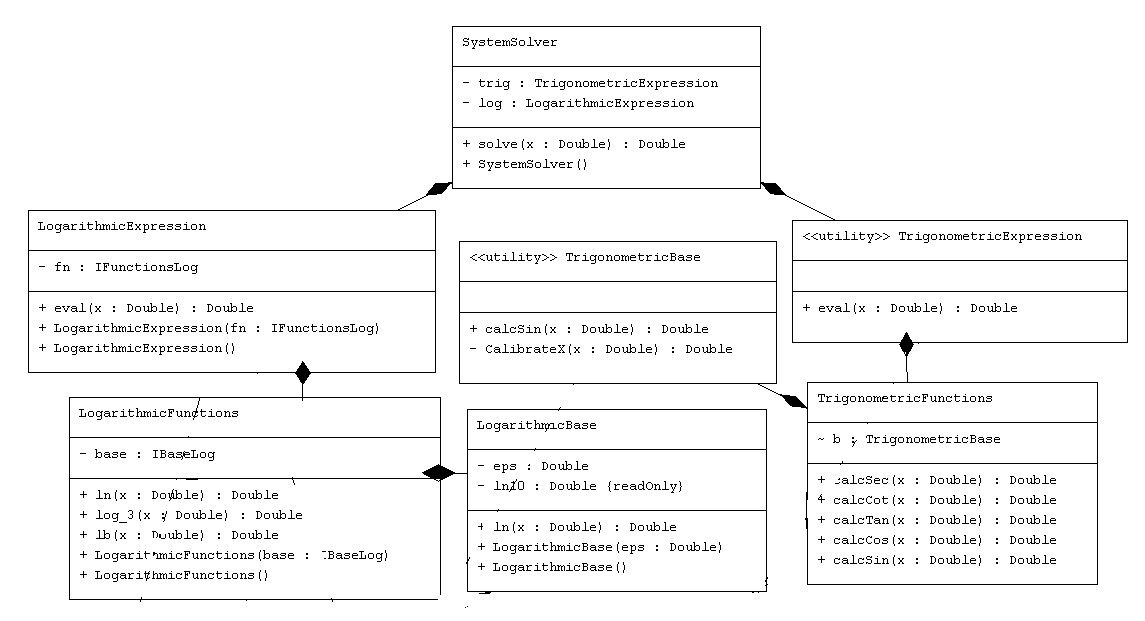
\includegraphics[scale=0.6]{./images/uml.jpg}
		\end{figure}
\section*{Тестовое покрытие}
    \subsection*{Модуль базовой функции $ln()$}
            \begin{tikzpicture}
                \begin{axis}[
                    domain=0.125:10,
                    xmin=0, xmax=7,
                    ymin=-5, ymax=5,
                    samples=500,
                    axis y line=center,
                    axis x line=middle,
					height = 5cm
                ]
                    \addplot+[mark=none] {ln(x)};
                \end{axis}
            \end{tikzpicture}

		Область определения функции $(0, \infty)$. 
		\begin{enumerate}
			\item $\forall x \in (0, 1), f(x) \in (-\infty, 0)$
			\item $\text{Для } x = 1, f(x) := 0$
			\item $\text{Для } x = e, f(x) := 1$
			\item $\forall x \in (1, \infty), f(x) \in (0, \infty)$
			\item $\forall x \in (-\infty, 0), f(x) \in \varnothing$
		\end{enumerate}

    \subsection*{Модуль логарифмических функций}
		\subsubsection*{$lb()$}
            \begin{tikzpicture}
                \begin{axis}[
                    domain=0.125:10,
                    xmin=0, xmax=7,
                    ymin=-5, ymax=5,
                    samples=500,
                    axis y line=center,
                    axis x line=middle,
					height = 5cm
                ]
                    \addplot+[mark=none] {ln(x)/ln(2)};
                \end{axis}
            \end{tikzpicture}

    		Функция выражена через натуральный логарифм: $lb(x) = ln(x)/ln(2)$.
    		Так как в данном модуле мы используем предположительно оттестированную функцию и математически обоснованное
    		преобразование функции, для тестирования функции двоичного логарифма достаточно оттестировать ряд значений,
    		являющихся степенью двойки.
		\subsubsection*{$log_3()$}
            \begin{tikzpicture}
                \begin{axis}[
                    domain=0.125:10,
                    xmin=0, xmax=7,
                    ymin=-5, ymax=5,
                    samples=500,
                    axis y line=center,
                    axis x line=middle,
					height = 5cm
                ]
                    \addplot+[mark=none] {ln(x)/ln(3)};
                \end{axis}
            \end{tikzpicture}
			Аналогично для логарифма по основанию 3.

    \subsection*{Модуль выражения с логарифмическими функциями}

		\begin{figure}[h!]
			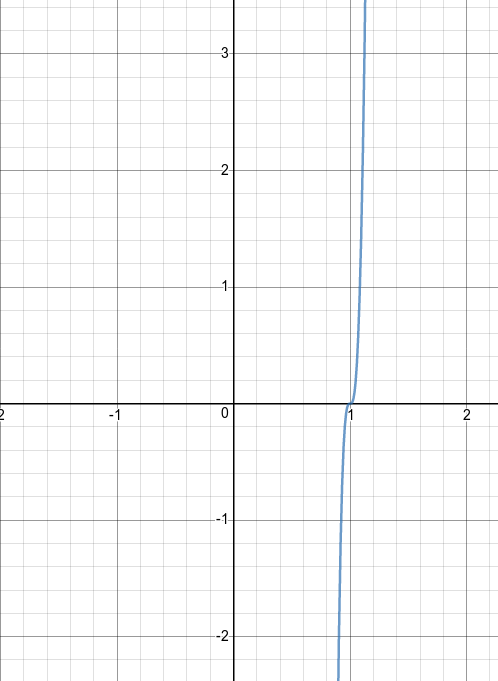
\includegraphics[scale=0.2]{./images/logExpr.png}
		\end{figure}
		Область определения функции $(0, \infty)$. 
		\begin{enumerate}
			\item $\forall x \in (0, 1), f(x) \in (-\infty, 0)$
			\item $\text{Для } x = 1, f(x) \in \varnothing$
			\item $\forall x \in (1, \infty), f(x) \in (0, \infty)$
			\item $\forall x \in (-\infty, 0), f(x) \in \varnothing$
		\end{enumerate}

    \subsection*{Модуль базовой функции $\sin()$}
            \begin{tikzpicture}
                \begin{axis}[
                    domain=-5:5,
                    xmin=-5, xmax=5,
                    ymin=-1, ymax=1,
                    samples=500,
                    axis y line=center,
                    axis x line=middle,
					height = 5cm
                ]
                    \addplot+[mark=none] {sin(deg(x))};
                \end{axis}
            \end{tikzpicture}
 Классы эквивалентности:
 \begin{enumerate}
 	\item $\sin(x) > 0 \forall x \in (2\pi n; \pi+2\pi n), n \in \mathbf Z$.
 	\item $\sin(x) < 0 \forall x \in (-\pi+2\pi n; 2\pi n), n \in \mathbf Z$.
 	\item Промежутки возрастания. $x \in (-\pi +2\pi n;\frac {\pi} {2}+2\pi n),    n \in z$.
 	\item Промежутки убывания. $x \in (- \frac {\pi} {2}+2\pi n;\frac {3\pi} {2}+2\pi n), n \in z$.
  \end{enumerate}
    \subsection*{Модуль тригонометрических функции} 
		\subsubsection*{Функция $\cos()$}
            \begin{tikzpicture}
                \begin{axis}[
                    domain=-5:5,
                    xmin=-5, xmax=5,
                    ymin=-1, ymax=1,
                    samples=500,
                    axis y line=center,
                    axis x line=middle,
					height = 5cm
                ]
                    \addplot+[mark=none] {cos(deg(x))};
                \end{axis}
            \end{tikzpicture}

	\begin{enumerate}
		\item  $\cos(x)>0, x \in (-\frac {\pi} {2}+2\pi n; \frac {\pi} {2}+2\pi n), n \in \mathbf Z$.
		\item  $\cos(x)<0, x \in (\frac {\pi} {2}+2\pi n;3\frac {\pi} {2}+2\pi n), n \in \mathbf Z$.
		\item  Промежутки возрастания. $x \in (-\pi+2\pi n;2\pi n), n \in \mathbf Z$.
		\item  Промежутки убывания. $x \in (2\pi n;\pi+2\pi n), n \in \mathbf Z$.
	\end{enumerate}
		\subsubsection*{Функция $\tan()$}
            \begin{tikzpicture}
                \begin{axis}[
                    domain=-2:2,
                    xmin=-2, xmax=2,
                    ymin=-5, ymax=5,
                    samples=500,
                    axis y line=center,
                    axis x line=middle,
					height = 5cm
                ]
                    \addplot+[mark=none] {tan(deg(x))};
                \end{axis}
            \end{tikzpicture}
			\begin{enumerate}
				\item  $(-\pi/2+2\pi n; \pi/2+2\pi n), n \in \mathbf Z$.
				\item  Точки разрыва $\frac {\pi} {2} + 2 \pi n, n \in \mathbf Z$.
			\end{enumerate}
       \subsubsection*{Функция $\cot()$}
            \begin{tikzpicture}
                \begin{axis}[
                    domain=-5:5,
                    xmin=-5, xmax=5,
                    ymin=-5, ymax=5,
                    samples=500,
                    axis y line=center,
                    axis x line=middle,
					height = 5cm
                ]
                    \addplot+[mark=none] {cot(deg(x))};
                \end{axis}
            \end{tikzpicture}
            \begin{enumerate}
                \item $(2\pi n; \pi+2\pi n), n \in \mathbf Z$.
                \item Точки разрыва $\pi+2 \pi n, n \in \mathbf Z$.
            \end{enumerate}
		\subsubsection*{Функция $\sec()$}
            \begin{tikzpicture}
                \begin{axis}[
                    domain=-5:5,
                    xmin=-5, xmax=5,
                    ymin=-5, ymax=5,
                    samples=500,
                    axis y line=center,
                    axis x line=middle,
					height = 5cm
                ]
                    \addplot+[mark=none] {sec(deg(x))};
                \end{axis}
            \end{tikzpicture}
		\begin{enumerate}
            \item $(-\frac {\pi} {2}+2\pi n; \frac {\pi} {2}+2\pi n), n \in \mathbf Z.$ 
            \item $(\frac {\pi} {2}+2\pi n;3\frac {\pi} {2}+2\pi n), n \in \mathbf Z.$ 
            \item Точки разрыва $\pi +2\pi n, n \in \mathbf Z$.
		\end{enumerate}

    \subsection*{Модуль выражения с тригонометрическими функциями}
		\begin{figure}[h!]
			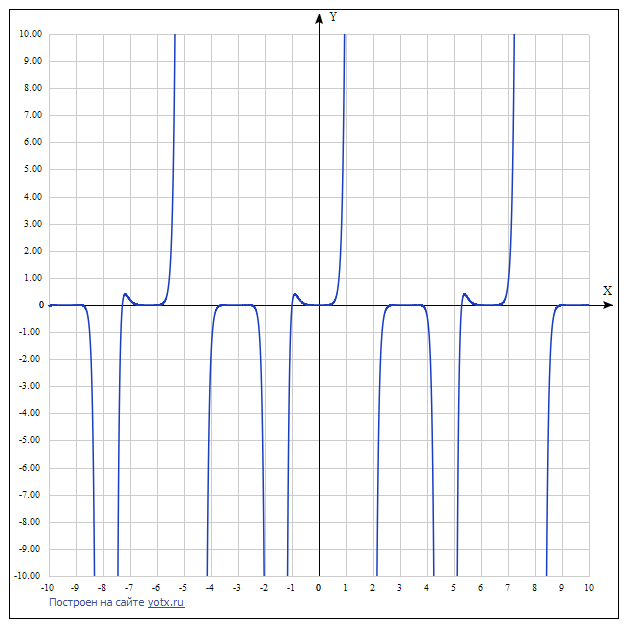
\includegraphics[scale=0.2]{./images/trigonometric_graphic.png}
		\end{figure}

    Для конечного неравенства системы были выделены следующие классы эквивалентности:
    \begin{enumerate}
    	\item $(-\frac \pi 2+2\pi n;\frac \pi 2+2\pi n), n \in \mathbf Z$.
    	\item $(\frac \pi 2+2\pi n;3\frac \pi 2+2\pi n), n \in \mathbf Z$.
    	\item Устранимые точки разрыва в $\pi n, n \in \mathbf Z$.
    	\item Разрывы второго рода в $\frac \pi 2 + \pi n$
    \end{enumerate}
\newpage
	\subsection*{Итогова система}
		\begin{figure}[h!]
			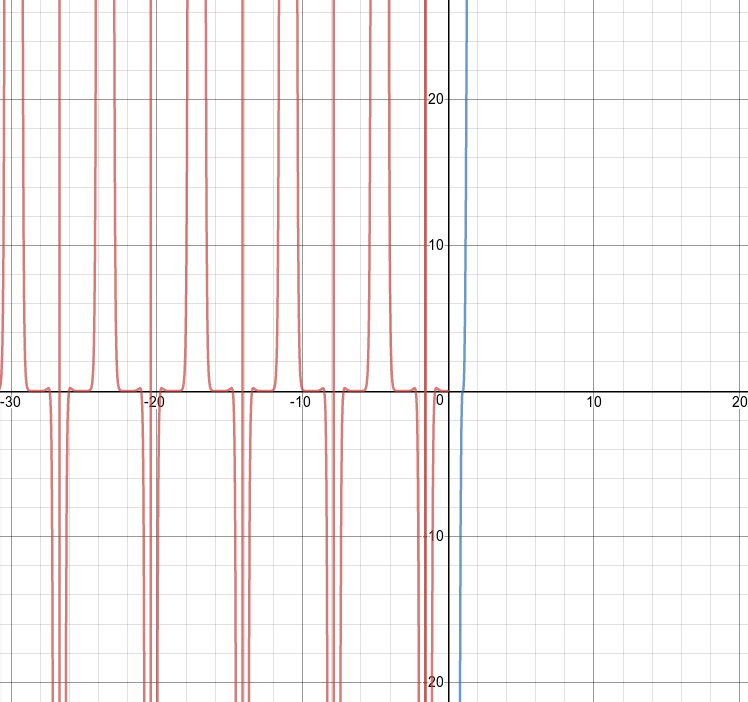
\includegraphics[scale=0.3]{./images/system.png}
		\end{figure}

		Тестовое покрытие аналогично тестовым покрытиям составляющих её функций на соответствующих диапазонах.
\section*{Вывод}
В ходе выполнения лабораторной работы была разработана архитектура проекта, реализующего
вычисление заданной системы функций. Было проведено модульное тестирование математических
модулей системы и проведенно интеграционное тестирование, в ходе которого были протестировано
взаимодействие модулей.
\end{document}
